% !TEX encoding = UTF-8 Unicode
% REMEMBER TO SET LANGUAGE!
\documentclass[a4paper,10pt,norsk]{article}
\usepackage[utf8]{inputenc}
\usepackage[norsk]{babel}
% Standard stuff
\usepackage{amsmath,graphicx,varioref,verbatim,amsfonts,geometry}
% colors in text
\usepackage[usenames,dvipsnames,svgnames,table]{xcolor}
% Hyper refs
\usepackage[colorlinks]{hyperref}

% Document formatting
\setlength{\parindent}{0mm}
\setlength{\parskip}{1.5mm}

%Color scheme for listings
\usepackage{textcomp}
\definecolor{listinggray}{gray}{0.9}
\definecolor{lbcolor}{rgb}{0.9,0.9,0.9}

%Listings configuration
\usepackage{listings}
%Hvis du bruker noe annet enn python, endre det her for å få riktig highlighting.
\lstset{
	backgroundcolor=\color{lbcolor},
	tabsize=4,
	rulecolor=,
	language=python,
        basicstyle=\scriptsize,
        upquote=true,
        aboveskip={1.5\baselineskip},
        columns=fixed,
	numbers=left,
        showstringspaces=false,
        extendedchars=true,
        breaklines=true,
        prebreak = \raisebox{0ex}[0ex][0ex]{\ensuremath{\hookleftarrow}},
        frame=single,
        showtabs=false,
        showspaces=false,
        showstringspaces=false,
        identifierstyle=\ttfamily,
        keywordstyle=\color[rgb]{0,0,1},
        commentstyle=\color[rgb]{0.133,0.545,0.133},
        stringstyle=\color[rgb]{0.627,0.126,0.941}
        }
        
\newcounter{subproject}
\renewcommand{\thesubproject}{\alph{subproject}}
\newenvironment{subproj}{
\begin{description}
\item[\refstepcounter{subproject}(\thesubproject)]
}{\end{description}}

%Lettering instead of numbering in different layers
%\renewcommand{\labelenumi}{\alph{enumi}}
\renewcommand{\thesubsection}{\alph{subsection}}

%opening
\title{MAT1110 - Oblig 1}
\author{Joakim Flatby}

\begin{document}

\maketitle
\section{}

%Oppg 1a
\subsection{)}

$T\left(\begin{matrix}2\\1\end{matrix}\right) = \left(\begin{matrix}-2\\1\end{matrix}\right)$

$T\left(\begin{matrix}1\\1\end{matrix}\right) = \left(\begin{matrix}1\\1\end{matrix}\right)$

Finn matrise A slik at $T_{x} = A_{x}$

\[T\left(\begin{matrix}2\\1\end{matrix}\right) = \left(\begin{matrix}a&c\\b&d\end{matrix}\right)\left(\begin{matrix}2\\1\end{matrix}\right) = \left(\begin{matrix}-2\\1\end{matrix}\right) = \left(\begin{matrix}2a + c\\2b + d\end{matrix}\right)\]
\[T\left(\begin{matrix}1\\1\end{matrix}\right) = \left(\begin{matrix}a&c\\b&d\end{matrix}\right)\left(\begin{matrix}1\\1\end{matrix}\right) = \left(\begin{matrix}1\\1\end{matrix}\right) = \left(\begin{matrix}a + c\\b + d\end{matrix}\right)\]

\[2a + c = -2\]
\[2b + d = 1\]

\[a + c = 1\]
\[b + d = 1\]

løser likningssett:

\[a = 1 - c\]
\[2(1-c) + c = -2\]
\[2 - c = -2\]
\[c = 4\]

\[a + 4 = 1\]
\[a = -3\]

\[b = 1 - d\]
\[2(1 - d) + d = 1\]
\[2 - d = 1\]
\[d = 1\]

\[b + 1 = 1\]
\[b = 0\]

putter verdiene for a, b, c og d inn i $\left(\begin{matrix}a&c\\b&d\end{matrix}\right)$

\[A = \left(\begin{matrix}-3&4\\0&1\end{matrix}\right)\]

%Oppg 1b
\subsection{)}

\[\lambda I_{2} \left(\begin{matrix}\lambda&0\\0&\lambda\end{matrix}\right)\]

For å finne egenverdiene tar vi identitetsmatrisen $\lambda I_{2}$, trekker fra $A$, og tar determinanten av resultatet:
 
\[det(\lambda - A) = det\left(\begin{matrix}\lambda + 3&-4\\0&\lambda - 1\end{matrix}\right)\]
\[ = (\lambda + 3)(\lambda - 1) \]
\[\Downarrow\]
\[\lambda_{1} = -3, \lambda_{2} = 1\]

\[Av_{1} = 3v_{1}\]

\[-3x + 4y = -3x\] 
\[\Downarrow\]
\[x = 1\]

\[y = -3y\]
\[\Downarrow\]
\[y = 0\]

\[v_{1} = \left(\begin{matrix} 1\\0 \end{matrix}\right)\]

\[Av_{2} = v_{2}\]

\[-3x+4y = x\]
\[\Downarrow\]
\[y = x\]

\[y = y\]
\[\Downarrow\]
\[x = 1, y = 1\]

\[v_{1} = \left(\begin{matrix} 1\\0 \end{matrix}\right), v_{2} = \left(\begin{matrix} 1\\1 \end{matrix}\right)\]

%Oppg 1c
\subsection{)}

\[A^{5}\left(\begin{matrix} 2\\1 \end{matrix}\right) + A^{3}\left(\begin{matrix} 2\\1 \end{matrix}\right) + A\left(\begin{matrix} 2\\1 \end{matrix}\right)\]

Det jeg gjør her er å skrive om $\left(\begin{matrix} 2\\1 \end{matrix}\right)$ til 

\[\left(\begin{matrix} 2\\1 \end{matrix}\right) = \left(\begin{matrix} 1\\0 \end{matrix}\right) + \left(\begin{matrix} 1\\1 \end{matrix}\right)\]

Og skriver om A med egenverdiene funnet i oppgave b,  så
\[A^{5}\left(\begin{matrix} 2\\1 \end{matrix}\right) + A^{3}\left(\begin{matrix} 2\\1 \end{matrix}\right) + A\left(\begin{matrix} 2\\1 \end{matrix}\right)\]
kan skrives om til:

\[\lambda_{1}^{5}\left(\begin{matrix} 1\\0 \end{matrix}\right) + \lambda_{2}^{5}\left(\begin{matrix} 1\\1 \end{matrix}\right) + \lambda_{1}^{3}\left(\begin{matrix} 1\\0 \end{matrix}\right) + \lambda_{2}^{3}\left(\begin{matrix} 1\\1 \end{matrix}\right) + \lambda_{1}\left(\begin{matrix} 1\\0 \end{matrix}\right) + \lambda_{2}\left(\begin{matrix} 1\\1 \end{matrix}\right)\]

og dermed blir verdiene som skal opphøyes skalare og oppgaven mye lettere å løse.

\[-3^{5}\left(\begin{matrix} 1\\0 \end{matrix}\right) + 1^{5}\left(\begin{matrix} 1\\1 \end{matrix}\right) - 3^{3}\left(\begin{matrix} 1\\0 \end{matrix}\right) + 1^{3}\left(\begin{matrix} 1\\1 \end{matrix}\right) - 3\left(\begin{matrix} 1\\0 \end{matrix}\right) + \left(\begin{matrix} 1\\1 \end{matrix}\right)\]

\[\left(\begin{matrix} -243\\0 \end{matrix}\right) + \left(\begin{matrix} 1\\1 \end{matrix}\right) - \left(\begin{matrix} 27\\0 \end{matrix}\right) + \left(\begin{matrix} 1\\1 \end{matrix}\right) - \left(\begin{matrix} 3\\0 \end{matrix}\right) + \left(\begin{matrix} 1\\1 \end{matrix}\right)\]

\[=\left(\begin{matrix} -270\\3 \end{matrix}\right)\]

%Oppgave 2
\section{}

%Oppg 2a
\subsection{)}

\begin{center}

\[s(x) = \left(\begin{matrix} x\\x^{2} \end{matrix}\right)\]
\[s'(x) = \left(\begin{matrix} 1\\2x \end{matrix}\right)\]

Normalvektor:
\[\left(\begin{matrix} 1\\2x \end{matrix}\right) \cdot \left(\begin{matrix} a\\b \end{matrix}\right) = 0\]

\[a + 2xb = 0\]
Velger b = -1
\[a - 2x = 0\]

\[a = 2x\]
\[b = -1\]

\[\vec{n}(x) = \left(\begin{matrix} 2x\\-1 \end{matrix}\right) \cdot \frac{1}{\sqrt{(2x)^{2} + (-1)^{2}}}\]

\[\vec{n} = \Bigg( \frac{2x}{\sqrt{4x^{2} + 1}}, \frac{-1}{\sqrt{4x^{2} + 1}} \Bigg)\]

\end{center}

%Oppg 2b
\subsection{)}
X og Y som funksjon av x:

Først finner jeg vektoren fra berøringspunktet til sentrum av sirkelen ved å gange enhetsnormalvektoren fra oppg $2a$ med $-\frac{1}{2}$

($\frac{1}{2}$ er radiusen i sirkelen, og ganger med -1 fordi normalvektoren fra oppgave 2a har negativ andrekonponent, mens vi nå trenger vektoren med positiv andrekomponent som peker inn i parabelen.)

$\rho = 1/2$

$(-n(x))\rho= \Big( \frac{2x}{\sqrt{4x^{2} + 1}}, \frac{-1}{\sqrt{4x^{2} + 1}} \Big) * -\frac{1}{2} = \Big( -\frac{x}{\sqrt{4x^{2} + 1}}, \frac{1}{2\sqrt{4x^{2} + 1}} \Big)$

Nå som vi har vektoren fra berøringspunktet til sentrum, kan vi addere dette med $s(x) = (x, x^{2})$

$ XY(x) = s(x) + (-n(x))\rho$

\[X(x) = x - \frac{x}{\sqrt{4x^{2} + 1}}\]

\[Y(x) = x^{2} + \frac{1}{2\sqrt{4x^{2} + 1}}\]

%Oppg 2c
\subsection{)}
Posisjonen til sentrum av kula er gitt ved X(x) og Y(x).

For å finne $\vec{v}(t)$ setter vi $x(t) = 2cos(t)$ inn i $X(x)$ og $Y(x)$ og deriverer med hensyn på t.

Tilsvarende for $\vec{a}(t)$, med dobbel derivasjon.

%Oppg 2d
\subsection{)}

Formel for buelengde:

$L(a, b) = \int_{a}^{b} \sqrt{x_{1}'^{2} + x_{2}'(t)^{2} + ... + x_{n}'(t)^{2}} dt$

s(t) gir:

\[x_{1} = t \Rightarrow x_{1}' = 1\]

\[x_{2} = t^{2} \Rightarrow x_{2}' = 2t\]

Bruker formelen for buelengde fra 0 til x, og setter $ t = \xi$

\[\sigma(x) = \int_{0}^{x} \sqrt{1 + 4\xi^{2}} d\xi\]

%Oppg 2e
\subsection{)}
$m(x) = r(x) - (X(x), Y(x))$. 

Dette er en vektor som har lengde og retning fra sentrum av disken til punktet $r(x)$. Punktet $r(x)$ roterer med klokka(relativt til sentrum av disken) når $x$ går i positiv retning. Vi kan forklare $m(x)$ med en rotasjonsmatrise der vi bruker vinkelen mellom vektoren som peker fra sentrum av kula til $r(x)$, og normalvektoren fra oppgave $2a$. Dermed har vi enhetsvektoren til $m(x)$, ganget med $\rho$ for å skalere med riktig lengde, som gjør at vi sitter igjen med en vektor som peker fra origo, i retningen til $r(x) - (X(x), Y(x))$, akkurat som oppgaven ba om.

%Oppg 2f
\subsection{)}

\lstinputlisting{oppg2f.py}

\begin{figure}[h!]
        \centering 
        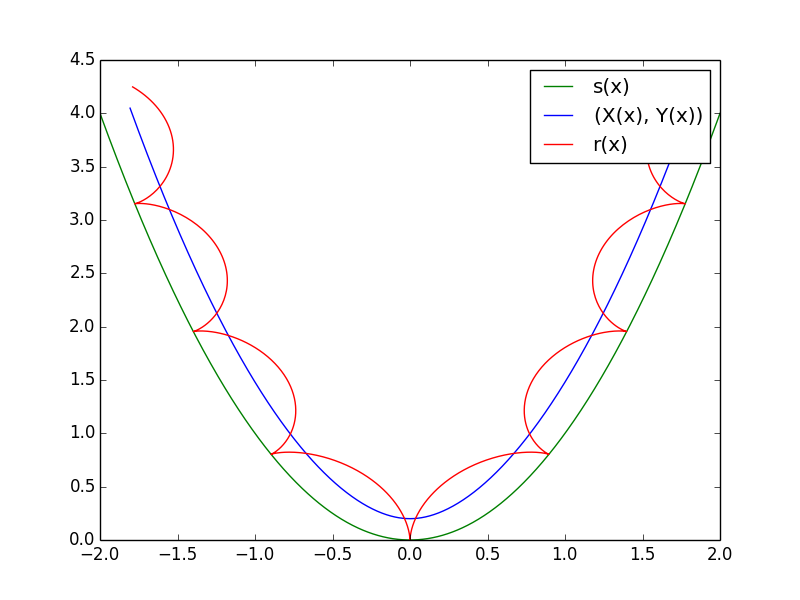
\includegraphics[scale=0.6]{oppg_f.png}
\end{figure}

\pagebreak

%oppg 3
\section{}
\subsection{)}

\begin{figure}[h!]
        \centering 
        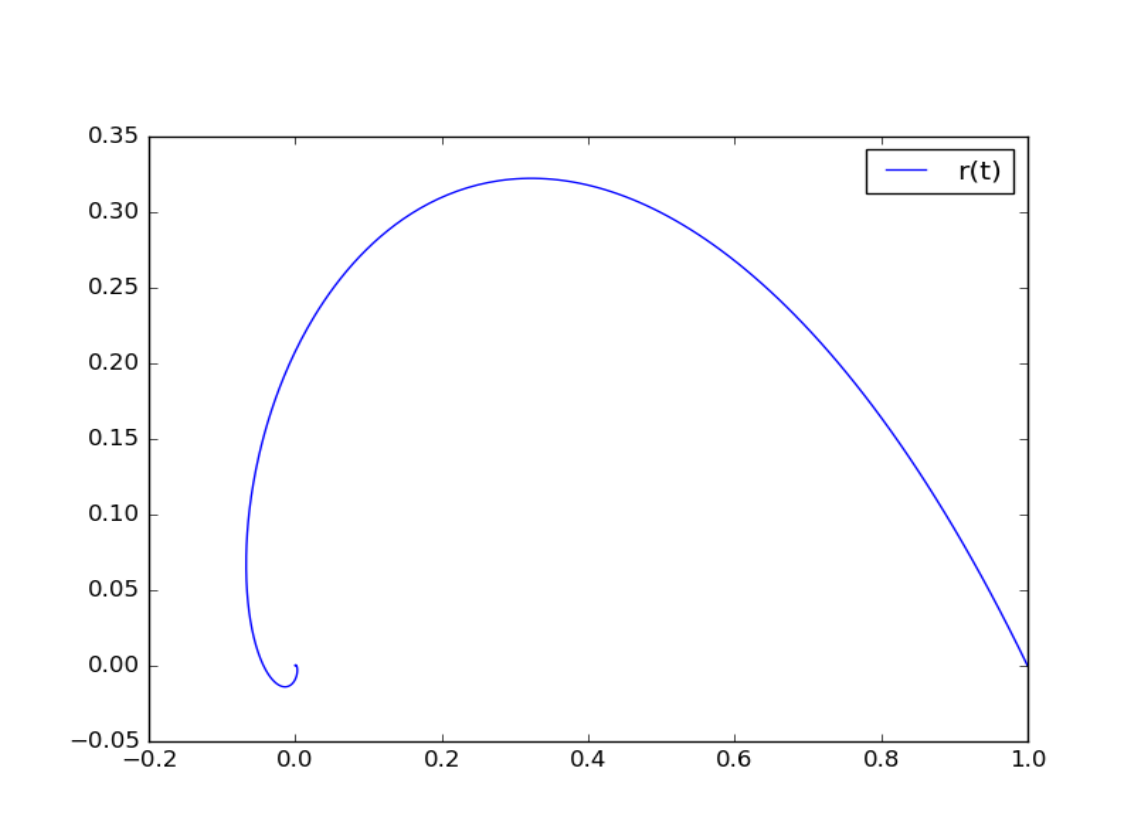
\includegraphics[scale=0.5]{skisse.png} 
        \caption{graphing r(t)}
\end{figure}

\pagebreak

%oppg 3b
\subsection{)}
r(t) er gitt ved $ r(t) = (e^{-t}cos(t), e^{-t}sin(t))$

Ved å derivere hvert komponent får vi:

$x'(t) = -e^{-t}cos(t) - e^{-t}sin(t)$

$y'(t) = -e^{-t}sin(t) + e^{-t}cos(t)$

Vet fra oppgave 2 d) at buelengden er:

$L(a, b) = \int_{a}^{b} \sqrt{x_{1}'^{2} + x_{2}'(t)^{2} + ... + x_{n}'(t)^{2}} dt$

Dermed får vi:

$L(0, \infty) = \int_{0}^{\infty} \sqrt{x'(t)^{2} + y'(t)^{2}} dt $

\[L(0, \infty) = \int_{0}^{\infty} \sqrt{(-e^{-t}cos(t) - e^{-t}sin(t))^{2} + (-e^{-t}sin(t) + e^{-t}cos(t))^{2}} dt \]
\[L(0, \infty) = \int_{0}^{\infty} \sqrt{2e^{-2t}(cos^{2}(t) + sin^{2}(t)} dt\]
\[L(0, \infty) = \int_{0}^{\infty} \sqrt{2e^{-2t}}dt\]
\[L(0, \infty) = \sqrt{2}\int_{0}^{\infty} \sqrt{e^{-t}}dt\]
\[L(0, \infty) = \sqrt{2}\Bigg( -e^{-\infty} + e^{0}\Bigg)\]
\[L(0, \infty) = \sqrt{2}\]

%oppg 3c
\subsection{)}

Har fra oppgave b:

$x'(t) = -e^{-t}cos(t) - e^{-t}sin(t)$

$y'(t) = -e^{-t}sin(t) + e^{-t}cos(t)$

Ved å skrive på vektorform får vi:

$\left(\begin{matrix} -e^{-t}cos(t)&-e^{-t}sin(t)\\e^{-t}cos(t)&-e^{-t}sin(t) \end{matrix}\right)$

Så kan vi trekke ut $r(t)$ og får:

$\left(\begin{matrix} -1&-1\\1&-1 \end{matrix}\right) * e^{-t}(cos(t)*\vec{i} + sin(t)*\vec{j})$

Dermed har vi svart på oppgaven ettersom dette kan skrives som:

$- \left(\begin{matrix} 1&1\\-1&1 \end{matrix}\right) * r(t)$

\section{}
%oppg 4a
\subsection{)}
Vis at $F$ er konservativt.

Må vise at funksjonen $\phi:\mathbb{R}^n \rightarrow \mathbb{R}$ finnes, slik at $\nabla \phi = \mathbf{F}$

Siden $f$ bare avhenger av $|x|$, så antar vi at $\phi$ også gjør det, og kan skrive:
$\phi(x) = g(|x|)$

Dermed har vi at:

\[\frac{\partial \phi}{\partial x_i} = \frac{\partial}{\partial x_i}g(|x|) = g'(|x|)\frac{\partial}{\partial x_i} \left(\sum_{i=1}^n x_i^2\right)^{\frac{1}{2}} = g'(|x|)\cdot 2x_i\cdot\frac{1}{2}\left(\sum_{i=1}^n x_i^2\right)^{-\frac{1}{2}} = \frac{g'(|x|)}{|x|} x_i\]

for $i = 1,\dots , n$

så,

\[\nabla \phi = \frac{g'(|x|)}{|x|}x.\]


Ettersom $f$ er kontinuerlig, så vet vi at det finnes en deriverbar funksjon:

$g: [0,\infty) \rightarrow \mathbb{R}$

slik at 

$g'(r) = rf(r)$

Vi vet også at $f'(r) \rightarrow 0$ når $r \rightarrow 0$, så dermed er $\lim_{r\rightarrow 0} f(r)$ veldefinert.

Dermad har vi:

\[\lim_{r \rightarrow 0} g'(r) = \lim_{r\rightarrow 0} rf(r) = 0\]
så:
\[\nabla \phi = \frac{g'(|x|)}{|x|}x\]
er veldefinert for $x=0$, og dermed er det bevist at $F$ er konservativt.

%oppg 4b
\subsection{)}

\[\nabla \phi(x) = \nabla h(|x|)\] 
\[= \sum_{i=1}^n \frac{\partial}{\partial x_i} h(|x|) e_i\]
hvor $e_i$ er enhetsvektoren til $x_i$
\[= \sum_{i=1}^n h'(|x|)\frac{\partial}{\partial x_i}\left(\sum_{j=1}^n x_j^2\right)^{\frac{1}{2}} e_i \]
\[= \sum_{i=1}^n |x| f(|x|)\text{ }2x_i\text{ }\frac{1}{2}\left(\sum_{j=1}^n x_j^2\right)^{-\frac{1}{2}} e_i \]
\[= \sum_{i=1}^n |x| f(|x|)\frac{1}{|x|}x_i e_i \]
\[=  \sum_{i=1}^n f(|x|) x_i e_i\]
\[= f(|x|)x\]
\[= \mathbf{F}(x)\]

som er det som skule vises.
\end{document}

